\chapter{network-flow}

	\textit{MESSAGE}
	\newline
	
	\begin{tabular}{ | l | l | l | l |}
		\hline
		ID & COUNT & VALUE & COMMITMENT \\
		\hline
		20 bits & 21 bits & 20 bits & 256 bits\\
		\hline
	\end{tabular}
	\newline
	\newline
	\textit{SIGNATURE (MESSAGE)}
	\newline

	\begin{tabular}{ |l| }
		\hline
		Encryption$_{secret-key_{node}}$( HASH ( MESSAGE ) )\\
		\hline
		500 bits\\
		\hline
	\end{tabular}
	\newline
	\newline
	\textit{CERTIFICATES}
	\newline

	\begin{tabular}{ | l | l | l | }
		\hline
			Public key  & Signature & ID \\
		\hline
			1000 bits & 500 bits & 20 bits \\
		\hline

	\end{tabular}
	\newline
	\newline
	\textit{NETWORK FLOW}
	\newline
	For the given aggregation tree, when a child communicates for the first time with its parent, it sends three things: Message, Signature of message \& Certificate. For any subsequent communications a child sends Message \& Signature of messsage. 

	\section{Star aggregation tree}

		In star aggregation topology root has to create ( n - 1 ) intermediate vertices, where n is the number of children root has.
		\textit{Note}: number of certificates = signatures = messages = public keys 	
	
	\begin{figure}[t]\label{star-aggregation-tree}
		\centering
			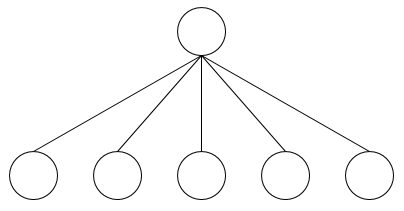
\includegraphics[width=0.7\textwidth]{images/star-aggregation-tree.png}\\
			\caption{Star aggregation tree}
	\end{figure}
	\begin{tabular}{ | l | l | l |}
		\hline
			\ & \#Messages & \#Certificates \\
		\hline
			To root	& O ( n ) & O ( n ) \\
		\hline
			From root & 1 & 1 \\
		\hline 
	\end{tabular}
		\newline
		\newline


If you have N children, each of your children has n cdescendent then following equality holds true:

$ N < number of certificates needed < N log(n) $